\begin{figure}%
  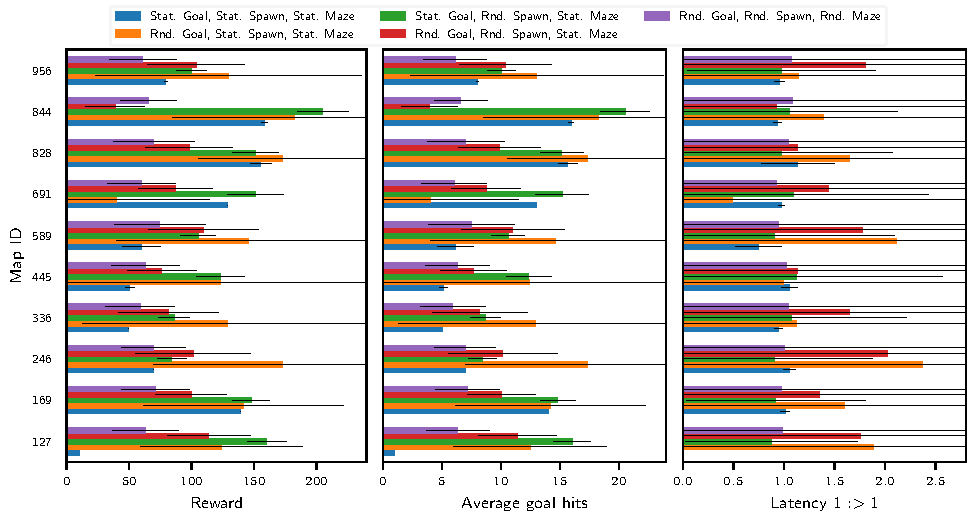
\includegraphics[width=\linewidth]{images/plot_summary_bar_plots.pdf}%
  \caption{
    We evaluate the \NavAiiiCDiDiiL{}~\cite{MiPaViICLR2017} algorithm on ten randomly chosen maps with increasing difficulty as described in Sec~\ref{sec:navtasks}.
    The figure is best viewed in color.
    Vertical axis is one of the ten maps on which the agent was trained and evaluated.
    Horizontal axis are different evaluation metrics.
    We note that when the goal is static then rewards are consistently higher as compared to random goal while static spawn location and random spawn location are roughly close to each other within bounds of uncertainity.
    With static goals, the metric Distance traveled : shortest path is close to 1,
    indicating that the algorithms are able to find shortest path. However, with random goals, the agents struggle to find the shortest path.
    From the \LatencyOneGtOne{} results we note that the current state of art algorithms do well when trained and tested on the same map but fail to generalize to new maps when evaluated on ability to exploit the information about goal location.
    Also note that \LatencyOneGtOne{} metric for cases of static goals is expected to be close to one because the location of goal is learned at train time.
  }%
\label{fig:latency-goal-reward}%
\end{figure}
